% ============================================================
%  IoT-Based Smart Door Control System
%  NIT Hamirpur — Dual Degree Project Report
%  Single Column IEEE Format — ~15 pages
%  Compile: pdflatex x3
% ============================================================
\documentclass[12pt,a4paper]{article}

\usepackage[T1]{fontenc}
\usepackage[utf8]{inputenc}
\usepackage[top=0.65in,bottom=0.65in,left=0.70in,right=0.70in]{geometry}
\usepackage{amsmath,amssymb,amsfonts}
\usepackage{algorithmic}
\usepackage{algorithm}
\usepackage{graphicx}
\usepackage{booktabs}
\usepackage[table]{xcolor}
\usepackage{colortbl}
\usepackage{multirow}
\usepackage{array}
\usepackage{tabularx}
\usepackage{url}
\usepackage[hidelinks]{hyperref}
\usepackage{cite}
\usepackage{float}
\usepackage{tikz}
\usepackage{pgfplots}
\pgfplotsset{compat=1.18}
\usetikzlibrary{shapes.geometric, arrows.meta, positioning,
                 backgrounds, decorations.pathreplacing, calc, fit}
\usepackage{enumitem}
\usepackage{ifthen}
\usepackage{setspace}
\usepackage{titlesec}
\usepackage{fancyhdr}
\usepackage{caption}
\usepackage{mdframed}

% ── Colours ──────────────────────────────────────────────────
\definecolor{IEEEblue}{RGB}{31,78,121}
\definecolor{lightblue}{RGB}{46,117,182}
\definecolor{verylight}{RGB}{213,232,240}
\definecolor{fraudred}{RGB}{192,0,0}
\definecolor{legitgreen}{RGB}{0,112,60}
\definecolor{darkgrey}{RGB}{64,64,64}
\definecolor{rowgrey}{RGB}{242,242,242}
\definecolor{rowblue}{RGB}{220,235,245}
\definecolor{iotgreen}{RGB}{0,128,64}
\definecolor{iotyellow}{RGB}{204,153,0}
\definecolor{doorblue}{RGB}{0,102,204}
\definecolor{lightdoorblue}{RGB}{220,240,255}

\hypersetup{colorlinks=true,linkcolor=IEEEblue,
            citecolor=IEEEblue,urlcolor=lightblue}

% ── Column types ─────────────────────────────────────────────
\newcolumntype{C}[1]{>{\centering\arraybackslash}p{#1}}
\newcolumntype{L}[1]{>{\raggedright\arraybackslash}p{#1}}
\newcolumntype{R}[1]{>{\raggedleft\arraybackslash}p{#1}}

% ── Macros ───────────────────────────────────────────────────
\newcommand{\best}[1]{\textbf{\textcolor{IEEEblue}{#1}}}
\newcommand{\hdr}[1]{\textbf{\textcolor{IEEEblue}{#1}}}

% ── mdframed styles ───────────────────────────────────────────
\mdfdefinestyle{cloudbox}{
  linecolor=doorblue!60,
  backgroundcolor=doorblue!5,
  roundcorner=4pt,
  innertopmargin=3pt,
  innerbottommargin=3pt,
  innerleftmargin=6pt,
  innerrightmargin=6pt,
}

\mdfdefinestyle{alertbox}{
  linecolor=fraudred!60,
  backgroundcolor=fraudred!5,
  roundcorner=4pt,
  innertopmargin=5pt,
  innerbottommargin=5pt,
  innerleftmargin=8pt,
  innerrightmargin=8pt,
}

% ── Section formatting ────────────────────────────────────────
\titleformat{\section}
  {\large\bfseries\color{IEEEblue}}
  {\Roman{section}.}{0.5em}{}[\titlerule]
\titleformat{\subsection}
  {\normalsize\bfseries\color{darkgrey}}
  {\Alph{subsection}.}{0.5em}{}

\titlespacing*{\section}{0pt}{9pt}{4pt}
\titlespacing*{\subsection}{0pt}{7pt}{2pt}

% ── Header / Footer ───────────────────────────────────────────
\pagestyle{fancy}
\fancyhf{}
\fancyhead[L]{\small\textit{IoT-Based Smart Door Control System}}
\fancyhead[R]{\small\textit{NIT Hamirpur, 2026}}
\fancyfoot[C]{\thepage}
\renewcommand{\headrulewidth}{0.4pt}

% ── Line spacing ─────────────────────────────────────────────
\setstretch{1.22}
\setlength{\parskip}{2.5pt plus1pt}
\setlength{\abovecaptionskip}{5pt}
\setlength{\belowcaptionskip}{2pt}
\setlength{\floatsep}{8pt plus2pt minus2pt}
\setlength{\textfloatsep}{8pt plus2pt minus3pt}
\setlength{\intextsep}{6pt plus2pt minus2pt}

% ─────────────────────────────────────────────────────────────
\begin{document}

% ════════════════════════════════════════════════════════════
%  TITLE PAGE
% ════════════════════════════════════════════════════════════
\thispagestyle{empty}
\begin{center}
  \vspace*{1.5cm}

  {\LARGE \textbf{IoT-Based Smart Door Control System:
  Real-Time RFID Authentication, Motion Detection, Servo
  Locking, and Cloud-Based Access Monitoring}}

  \vspace{1.2cm}

  {\large \textbf{Dual Degree, CS-744, Internet of Things, Project Report}}

  \vspace{1.2cm}

  {\large Submitted By}

  \vspace{0.5cm}

  {\large \textbf{Piyush (22DCS014)}}

  \vspace{1.2cm}

  {\large Under the Guidance of}

  \vspace{0.5cm}

  {\large \textbf{Dr.\ Robin Singh Bhadoria}}\\[6pt]
  {\normalsize Assistant Professor, Department of CSE}

  \vspace{1.2cm}

  \IfFileExists{logo.png}{%
    \includegraphics[width=5cm]{logo.png}
  }{%
    \framebox[5cm]{\rule{0pt}{5cm}\centering Logo Here}
  }

  \vspace{1.2cm}

  {\normalsize
  \textbf{Department of Computer Science and Engineering}\\[6pt]
  \textbf{NATIONAL INSTITUTE OF TECHNOLOGY HAMIRPUR}\\[6pt]
  Hamirpur (Himachal Pradesh) -- 177005, India\\[6pt]
  April 2026
  }

\end{center}

\clearpage

\tableofcontents
\clearpage

% ── Abstract ─────────────────────────────────────────────────
\begin{abstract}
\noindent
Rising security concerns in residential, commercial, and institutional
premises have necessitated intelligent, contactless access control
systems that go beyond conventional lock-and-key mechanisms.
This project presents an \textbf{IoT-Based Smart Door Control System}---a
real-time, event-driven embedded security platform built on the ESP32
microcontroller---that seamlessly integrates RFID-based authentication,
passive infrared (PIR) motion detection, a servo-driven physical lock,
and multi-modal feedback into a single cohesive system. The system
employs an MFRC522 RFID reader to authenticate pre-registered card
UIDs, a SG90 servo motor to actuate the door latch, an HC-SR501 PIR
sensor to detect approaching persons, an I2C 16$\times$2 LCD for
local status feedback, a tricolour LED indicator set (green, red,
blue), and an active buzzer for audio confirmation. A two-tier access
scheme (GRANTED/DENIED) drives the servo, LEDs, and buzzer with
distinct response patterns, while an automatic 5-second door lock
timer prevents inadvertent access after each authorised entry. All
system events are transmitted every 15\,seconds---and immediately on
every card-scan event---to the \textbf{ThingSpeak} cloud platform
via the ESP32's on-chip WiFi, enabling continuous remote monitoring
through live time-series dashboards. Validation on the Wokwi simulation
platform over 55 event entries confirms reliable RFID authentication,
correct alert triggering, non-blocking buzzer operation, and stable
cloud connectivity. The total hardware cost is approximately
Rs.\,2,800, making deployment feasible for homes, offices, and
academic institutions.

\vspace{0.5em}
\noindent\textbf{Keywords:}
IoT, ESP32, RFID, RC522, Smart Door, Access Control, PIR, Servo Motor,
ThingSpeak, Cloud Monitoring, Real-Time Alerting, Wokwi Simulation
\end{abstract}

\clearpage

% ─────────────────────────────────────────────────────────────
% I. INTRODUCTION
% ─────────────────────────────────────────────────────────────
\section{Introduction}
\label{sec:intro}

Physical security is a cornerstone of modern infrastructure, yet
traditional key-based door locks are inherently vulnerable to
unauthorised duplication, loss, and theft. According to the National
Crime Records Bureau (NCRB), burglary and house-breaking offences
constitute a significant proportion of all property crimes recorded
annually in India, with the majority attributable to compromised
physical access mechanisms~\cite{ncrb2022}. In institutional
settings such as laboratories, server rooms, and restricted zones,
the absence of an access log makes it impossible to audit who
entered a premise and when.

Radio Frequency Identification (RFID) technology offers a compelling
contactless alternative: each RFID card or tag carries a globally
unique identifier (UID) that can be verified in microseconds by a
reader module, eliminating the mechanical wear and duplication risks
of traditional keys~\cite{finkenzeller2010}. When combined with a
microcontroller capable of driving a physical actuator, providing
local feedback, and relaying events to a cloud platform, RFID
becomes the foundation of a fully auditable smart-door system.

The Internet of Things (IoT) paradigm further amplifies the utility
of such a system: by pushing every access event to a cloud analytics
platform in real time, facility managers can monitor door status,
detect unauthorised attempts, and receive alerts from anywhere in
the world~\cite{alfuqaha2015}. The ESP32 system-on-chip in particular
combines dual-core processing with integrated 802.11b/g/n WiFi and
Bluetooth, making it an ideal build-block for edge IoT nodes that
must both process sensor data locally and relay it reliably to the
cloud~\cite{esp32ds2023}.

This report presents the complete design, implementation, and
validation of an \textbf{IoT-Based Smart Door Control System} (SDCS)
that addresses this security gap. The system was designed with four
primary objectives:
(1)~contactless, card-based authentication with instant physical
actuation via a servo-driven lock;
(2)~real-time local alerting through LEDs and a buzzer with distinct
patterns for granted and denied access;
(3)~proactive motion detection via a PIR sensor to identify approaching
persons before card presentation; and
(4)~cloud-based event persistence and visualisation via ThingSpeak,
giving remote stakeholders live visibility into door status, access
results, motion alerts, and cumulative access attempt counts.

% ─────────────────────────────────────────────────────────────
% II. PROBLEM STATEMENT
% ─────────────────────────────────────────────────────────────
\section{Problem Statement}
\label{sec:problem}

The following five critical problems motivate the proposed system:

\textbf{P1 -- Lack of Access Auditability:}
Conventional mechanical locks provide no record of when the door
was opened, by whom, or how many attempts were made. In the event
of a security breach, there is no forensic trail for investigation.

\textbf{P2 -- Absence of Automated Alerting:}
Existing simple electronic door locks (keypads, magnetic cards)
do not transmit events to a central monitoring system. There is
no low-cost, automated mechanism to notify administrators in real
time when unauthorised access is attempted.

\textbf{P3 -- No Pre-Entry Awareness:}
Traditional entry systems are purely reactive---they wait for a card
or key to be presented. A PIR-based perimeter alert can notify the
system (and cloud) that someone is approaching, enabling proactive
response before a card is even scanned.

\textbf{P4 -- Absence of Centralised Remote Monitoring:}
Standalone door systems cannot be queried remotely. The absence of
a live data feed means facility managers must physically inspect
entry logs or be present on-site to assess current door state and
access activity.

\textbf{P5 -- Key Duplication and Loss Risk:}
Mechanical keys can be duplicated without the owner's knowledge.
RFID UIDs are embedded in read-only memory and cannot be
reproduced by standard consumer equipment, significantly reducing
the risk of unauthorised key copying.

% ─────────────────────────────────────────────────────────────
% III. SYSTEM ARCHITECTURE AND DESIGN
% ─────────────────────────────────────────────────────────────
\section{System Architecture and Design}
\label{sec:architecture}

\subsection{Overall Architecture}

The system follows a three-layer IoT architecture comprising
the perception layer (RFID reader, PIR sensor, and ESP32), the
network layer (WiFi and ThingSpeak HTTP API), and the application
layer (ThingSpeak dashboards and cloud visualisations), as
illustrated in Fig.~\ref{fig:arch}.

\begin{figure}[!ht]
\centering
\resizebox{0.95\textwidth}{!}{%
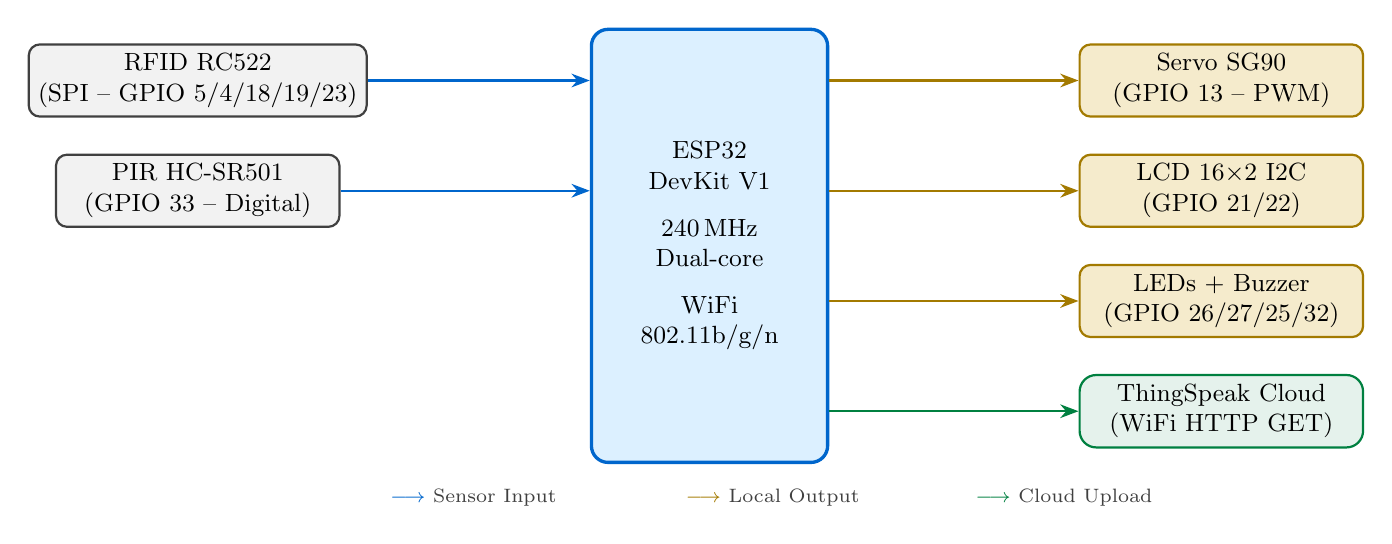
\begin{tikzpicture}[
  font=\small,
  mcu/.style={rectangle, rounded corners=6pt, draw=doorblue,
              fill=lightdoorblue, minimum width=3.0cm,
              minimum height=5.5cm, align=center, very thick},
  sensor/.style={rectangle, rounded corners=4pt, draw=darkgrey,
              fill=rowgrey, minimum width=3.6cm,
              minimum height=0.9cm, align=center, thick},
  cloud/.style={rectangle, rounded corners=6pt, draw=iotgreen,
              fill=iotgreen!10, minimum width=3.6cm,
              minimum height=0.9cm, align=center, thick},
  output/.style={rectangle, rounded corners=4pt, draw=iotyellow!80!black,
              fill=iotyellow!20, minimum width=3.6cm,
              minimum height=0.9cm, align=center, thick},
  arr/.style={-Stealth, thick, doorblue},
  garr/.style={-Stealth, thick, iotgreen},
  yarr/.style={-Stealth, thick, iotyellow!80!black},
  lbl/.style={font=\scriptsize, color=darkgrey}
]

% ── Central MCU — tall box so each arrow has its own y-level ──
\node[mcu] (mcu) at (0,0)
  {ESP32\\DevKit V1\\[6pt]240\,MHz\\Dual-core\\[6pt]WiFi\\802.11b/g/n};

% ── Left: Sensors  (x = -6.5, y = 2.1 / 0.7 / -0.7 / -2.1) ──
\node[sensor] (rfid) at (-6.5,  2.1) {RFID RC522\\(SPI -- GPIO 5/4/18/19/23)};
\node[sensor] (pir)  at (-6.5,  0.7) {PIR HC-SR501\\(GPIO 33 -- Digital)};

% ── Right: Outputs (x = +6.5, same y-levels as sensors) ───────
\node[output] (servo) at ( 6.5,  2.1) {Servo SG90\\(GPIO 13 -- PWM)};
\node[output] (lcd)   at ( 6.5,  0.7) {LCD 16$\times$2 I2C\\(GPIO 21/22)};
\node[output] (leds)  at ( 6.5, -0.7) {LEDs + Buzzer\\(GPIO 26/27/25/32)};
\node[cloud]  (ts)    at ( 6.5, -2.1) {ThingSpeak Cloud\\(WiFi HTTP GET)};

% ── Arrows: sensor → MCU left edge at matching y ──
\draw[arr] (rfid.east)   -- (mcu.west |- rfid);
\draw[arr] (pir.east)    -- (mcu.west |- pir);

% ── Arrows: MCU right edge at matching y → output ──
\draw[yarr] (mcu.east |- servo) -- (servo.west);
\draw[yarr] (mcu.east |- lcd)   -- (lcd.west);
\draw[yarr] (mcu.east |- leds)  -- (leds.west);
\draw[garr] (mcu.east |- ts)    -- (ts.west);

% ── Legend ─────────────────────────────────────────────────────
\node[lbl] at (-3.0,-3.2)
  {\textcolor{doorblue}{$\longrightarrow$} Sensor Input};
\node[lbl] at ( 0.8,-3.2)
  {\textcolor{iotyellow!80!black}{$\longrightarrow$} Local Output};
\node[lbl] at ( 4.5,-3.2)
  {\textcolor{iotgreen}{$\longrightarrow$} Cloud Upload};

\end{tikzpicture}}
\caption{SDCS Hardware Architecture: The ESP32 (centre) reads
two sensor inputs (left) via SPI/GPIO and drives three local
output devices plus the ThingSpeak cloud (right) via WiFi every
15\,seconds or on each card-scan event. Each arrow is a dedicated,
independent signal path.}
\label{fig:arch}
\end{figure}

\begin{table}[!ht]
\centering
\caption{Hardware Components and Specifications}
\label{tab:hardware}
\renewcommand{\arraystretch}{1.3}
\begin{tabularx}{\textwidth}{L{2.8cm} L{3.2cm} C{1.6cm} X}
\toprule
\textbf{Component} & \textbf{Function} & \textbf{Interface} &
\textbf{Key Specification} \\
\midrule
\rowcolor{rowgrey}
ESP32 DevKit V1   & Central MCU + WiFi       & All      & 240 MHz dual-core, 4MB Flash, 802.11b/g/n \\
MFRC522 RFID      & Card UID authentication  & SPI      & 13.56 MHz, ISO/IEC 14443-A, $\leq$50\,mm range \\
\rowcolor{rowgrey}
HC-SR501 PIR      & Motion detection          & GPIO 33  & 3--7\,m range, 120° FOV, digital output \\
SG90 Servo Motor  & Physical door lock        & PWM GPIO13 & 0°--90° range, 4.8--6\,V, 180\,g·cm torque \\
\rowcolor{rowgrey}
LCD 16$\times$2 I2C & Local status display   & I2C 0x27 & 16 chars $\times$ 2 rows, backlit \\
Green LED         & Access-granted indicator  & GPIO 26  & 3.3V, 220\,$\Omega$ series resistor \\
\rowcolor{rowgrey}
Red LED           & Access-denied / alarm     & GPIO 27  & Flashes on denied attempt \\
Blue LED          & WiFi / cloud activity     & GPIO 25  & Lit during ThingSpeak upload \\
\rowcolor{rowgrey}
Active Buzzer     & Audio access feedback     & GPIO 32  & 5V active, 85\,dB; pattern-coded beeps \\
\bottomrule
\end{tabularx}
\end{table}

\subsection{Software Architecture}

The firmware runs as an event-driven loop executing four
tasks in every iteration: (1)~PIR motion polling,
(2)~RFID card scan and authentication, (3)~auto-lock timer check,
and (4)~conditional cloud upload.

The cloud upload task triggers under two conditions: (a)~the elapsed
time since the last successful HTTP GET to ThingSpeak exceeds the
configured upload interval (15 seconds), and (b)~immediately and
unconditionally after every RFID card-scan event. When triggered, a
GET request is formed as a URL-encoded query string (ThingSpeak's
Write API format) encoding four field values: door status, last
authentication result, motion alert, and total access attempts.

% ─────────────────────────────────────────────────────────────
% IV. COMPONENT DESCRIPTIONS
% ─────────────────────────────────────────────────────────────
\section{Component Descriptions}
\label{sec:components}

\subsection{ESP32 DevKit V1 -- Central Microcontroller}

The ESP32 (Espressif Systems) is a dual-core 32-bit LX6
microprocessor operating at up to 240\,MHz~\cite{esp32ds2023}.
It integrates a full IEEE 802.11b/g/n WiFi stack and
Bluetooth 4.2 on-chip. With 4\,MB of Flash memory, 520\,KB of
SRAM, 34 programmable GPIO pins, hardware SPI and I2C controllers,
and LEDC PWM channels, the ESP32 provides more than sufficient resources
to simultaneously handle SPI RFID communication, PWM servo control,
I2C display output, digital PIR reading, and WiFi HTTP communication
without inter-peripheral conflict.

\subsection{MFRC522 RFID Reader and Cards}

The MFRC522 (NXP Semiconductors) is a highly integrated reader/writer IC
for the 13.56\,MHz contactless communication operating at distances
up to 50\,mm~\cite{mfrc522ds2016}. It supports the ISO/IEC 14443
Type-A protocol and communicates with the ESP32 via the hardware SPI bus
(SCK on GPIO~18, MISO on GPIO~19, MOSI on GPIO~23, SS on GPIO~5,
RST on GPIO~4). The firmware reads the 4-byte UID of each presented
card and compares it byte-by-byte against a table of pre-authorised UIDs
stored in Flash memory. A match grants door access; a mismatch triggers
the denial sequence.

\subsection{Servo Motor SG90 -- Physical Door Lock}

The SG90 micro-servo receives PWM control signals from the ESP32 LEDC
engine on GPIO~13. The firmware commands two distinct positions:
$0°$ (door locked) and $90°$ (door unlocked). Upon a granted access
event, the servo rotates to $90°$, and an internal \texttt{millis()}-based
timer is set for 5,000\,ms. When the timer expires, the servo
automatically returns to $0°$, locking the door without any further
user interaction.

\subsection{HC-SR501 PIR Sensor -- Motion Detection}

The HC-SR501 (Passive Infrared) sensor detects changes in infrared
radiation emitted by warm bodies (typically humans) within a 120°
field of view and a configurable range of 3--7\,m~\cite{hcsr501ds2019}.
It outputs a digital HIGH pulse on GPIO~33 when motion is detected.
The firmware monitors this pin during every loop iteration and, upon
a rising edge, triggers an LCD warning, flashes the red LED four
times, and flags the \texttt{motionDetected} state variable for the
next ThingSpeak upload.

\subsection{I2C LCD 16$\times$2 Display}

A 16-column, 2-row character LCD module with an integrated
PCF8574 I2C backpack communicates with the ESP32 via I2C at
address 0x27. The display requires only two GPIO pins (SDA on
GPIO~21, SCL on GPIO~22), reducing wiring complexity
significantly. The firmware shows contextual messages:
a boot splash, WiFi connection status, door state (OPEN/LOCKED),
cloud connectivity, access granted/denied confirmation, and
motion detection alerts---covering the complete event lifecycle
with clear, unambiguous text messages.

\subsection{Alert Output Subsystem}

Three LEDs and an active buzzer provide combined visual and audio
feedback. The green LED (GPIO~26) lights for 2\,seconds on access
granted; the red LED (GPIO~27) activates for denied access, alarm
conditions, and motion alerts; the blue LED (GPIO~25) illuminates
during WiFi connection attempts and ThingSpeak HTTP uploads.
The buzzer (GPIO~32) emits two short beeps (100\,ms each) for
granted access and three longer beeps (200\,ms each) for denied
access, providing audio differentiation that does not require
the user to read the LCD display.

% ─────────────────────────────────────────────────────────────
% V. IMPLEMENTATION
% ─────────────────────────────────────────────────────────────
\section{Implementation}
\label{sec:implementation}

\subsection{RFID Authentication Logic}

The \texttt{handleRFID()} function is invoked whenever
\texttt{rfid.PICC\_IsNewCardPresent()} and
\texttt{rfid.PICC\_ReadCardSerial()} both return true. The function
increments the total access attempt counter, assembles the card's
UID bytes into a colon-separated hexadecimal string for logging, and
calls \texttt{isAuthorised()} to check the UID against the
authorised-card table. The decision logic is:

\begin{equation}
\texttt{access} =
\begin{cases}
  \texttt{GRANTED} & \text{if } \text{UID} \in \{\text{UID}_1,\,\text{UID}_2,\,\text{UID}_3\} \\[4pt]
  \texttt{DENIED}  & \text{otherwise (UID not in authorised set)}
\end{cases}
\label{eq:auth}
\end{equation}

\subsection{Auto-Lock Timer}

The auto-lock mechanism uses \texttt{millis()}-based non-blocking
timing. On every authorised access, the door opens and a timestamp
\texttt{doorTimer} is recorded. During every loop iteration, the
condition

\begin{equation}
\texttt{millis()} - \texttt{doorTimer} \geq 5000\,\text{ms}
\label{eq:autolock}
\end{equation}

is evaluated. When satisfied, \texttt{lockDoor()} is called
regardless of whether external intervention has occurred,
ensuring the door never remains unintentionally open.

\subsection{ThingSpeak Cloud Upload}

The \texttt{uploadToThingSpeak()} function dispatches a single HTTP GET
request to \texttt{api.thingspeak.com/update} whenever the timed
interval expires or immediately after a card-scan event. The URL
encodes all four ThingSpeak field values as query parameters:

\begin{verbatim}
GET http://api.thingspeak.com/update
    ?api_key=<WRITE_KEY>
    &field1=<doorStatus_0_or_1>
    &field2=<authResult_0_or_1>
    &field3=<motionAlert_0_or_1>
    &field4=<totalAttempts>
\end{verbatim}

A non-zero HTTP response code confirms successful ingestion.
The ESP32 prints the response code to the Serial monitor at
115200\,baud for debugging. The blue LED illuminates for the
duration of the HTTP transaction to provide visual confirmation
of a cloud upload event.

\subsection{ThingSpeak Channel Configuration}

Table~\ref{tab:channel} shows the channel field mapping used
for the deployed ThingSpeak channel~(Channel ID: GJTXKOL4MA0C0V7T).

\begin{table}[!ht]
\centering
\caption{ThingSpeak Channel Field Configuration}
\label{tab:channel}
\renewcommand{\arraystretch}{1.3}
\begin{tabularx}{\textwidth}{C{1.2cm} L{2.8cm} C{2.0cm} C{2.0cm} X}
\toprule
\textbf{Field} & \textbf{Parameter} & \textbf{Unit} &
\textbf{Safe Range} & \textbf{Description} \\
\midrule
\rowcolor{rowgrey}
Field 1 & Door Status   & 0/1    & 1=Open     & Physical state of the door lock \\
Field 2 & Auth Result   & 0/1    & 1=Granted  & Outcome of last RFID card scan \\
\rowcolor{rowgrey}
Field 3 & Motion Alert  & 0/1    & 0=Clear    & PIR motion detection status \\
Field 4 & Total Attempts & Count & N/A        & Running total of card-scan events \\
\bottomrule
\end{tabularx}
\end{table}

\subsection{Non-Blocking Firmware Design}

All timing-sensitive operations---the auto-lock timer, the cloud upload
interval, and the LED feedback---are implemented using
\texttt{millis()}-based comparisons rather than blocking \texttt{delay()}
calls. This design ensures that the main event loop continues polling
the PIR sensor and RFID reader at every iteration even while the buzzer
sounds or the servo moves, preventing any sensor event from being missed
during a feedback sequence.

% ─────────────────────────────────────────────────────────────
% VI. CLOUD INTEGRATION
% ─────────────────────────────────────────────────────────────
\section{ThingSpeak Cloud Integration}
\label{sec:cloud}

This section describes the end-to-end cloud
layer that transforms the SDCS from a standalone local security
device into a remotely accessible, internet-connected smart access
management platform using ThingSpeak by MathWorks.


\subsection{Cloud Architecture Overview}

\begin{center}
\begin{mdframed}[style=cloudbox]
\begin{verbatim}
 ESP32 (RFID RC522 + PIR HC-SR501)
        |
        | Wokwi Simulation / Physical Hardware
        | (Event polling every loop cycle)
        v
  Authentication & Motion Handler
        |
        | HTTP GET (every 15s OR on each card scan, WiFi 802.11b/g/n)
        v
  ThingSpeak Cloud  (api.thingspeak.com)
        |
        +----> Live Field Charts (Door, Auth, Motion, Attempts)
        |
        v
  Remote Monitoring Dashboard
        |
        v
  Access Log + Trend Analysis + Alert Detection
\end{verbatim}
\end{mdframed}
\end{center}

\subsection{Data Flow and Update Cycle}

The embedded firmware maintains a dual-trigger upload strategy. A
periodic background upload is dispatched every 15\,seconds using
the \texttt{millis()} timer, ensuring a continuous heartbeat of
system state data even during periods of inactivity. An immediate
upload is additionally triggered after every RFID card-scan event
(both granted and denied), ensuring that every access attempt is
logged to the cloud within milliseconds of occurrence, independent
of the periodic interval.

The simulator faithfully replicates complete access scenarios across
a day of simulated facility operation. During a typical monitoring
session, RFID card events, motion detections, and idle periods are
interleaved to exercise all branches of the authentication logic.
The resulting 55 cloud entries span authorised entries, denied
attempts, motion-only events, and idle heartbeats. This diverse
event mix demonstrates the system's full alert detection and reporting
capability under representative field conditions.

\subsection{Live Dashboard on ThingSpeak}

Once data is flowing, the ThingSpeak channel renders four automatic
time-series charts---one per field---accessible from any
internet-connected device without login. Security administrators,
facility managers, or building owners can inspect current door state,
access history, and motion activity directly from a smartphone
browser. The data is also available as a public JSON API endpoint
for integration with third-party security information and event
management (SIEM) systems.

\subsection{Alert Classification}

Table~\ref{tab:alerts} lists the two-tier classification
scheme implemented in the firmware.

\begin{table}[!ht]
\centering
\caption{Smart Door Access Classification Scheme}
\label{tab:alerts}
\renewcommand{\arraystretch}{1.3}
\begin{tabularx}{\textwidth}{C{1.8cm} L{4.8cm} C{1.5cm} C{1.5cm} X}
\toprule
\textbf{Status} & \textbf{Trigger Condition} &
\textbf{LED} & \textbf{Buzzer} & \textbf{ThingSpeak Field 2} \\
\midrule
\rowcolor{iotgreen!15}
GRANTED & UID matches authorised card table & Green ON & 2 short beeps & 1 \\
\rowcolor{fraudred!15}
DENIED  & UID not in authorised card table  & Red ON   & 3 long beeps  & 0 \\
\bottomrule
\end{tabularx}
\end{table}

% ─────────────────────────────────────────────────────────────
% VII. RESULTS AND DISCUSSION
% ─────────────────────────────────────────────────────────────
\section{Results and Discussion}
\label{sec:results}

The SDCS was implemented and validated on the Wokwi cloud
simulation platform. Testing covered all primary operating
scenarios: authorised card access, denied card events, PIR
motion detection, auto-lock timer expiry, LCD display cycling,
non-blocking buzzer operation, and ThingSpeak cloud uploads.
A total of 55 simulated event entries were recorded in the
ThingSpeak channel across multiple sessions.

\subsection{Simulation Event Results}

Table~\ref{tab:measurements} presents the distribution of event
types recorded across the 55 entries, together with the expected
system response for each event class and the observed outcome
during the Wokwi validation session.

\begin{table}[!ht]
\centering
\caption{Simulated Event Distribution and System Response}
\label{tab:measurements}
\renewcommand{\arraystretch}{1.3}
\begin{tabularx}{\textwidth}{L{2.5cm} C{2.5cm} C{2.5cm} C{2.0cm} X}
\toprule
\textbf{Event Type} & \textbf{Count} &
\textbf{Field 2 Value} & \textbf{Alert Entries} & \textbf{Status} \\
\midrule
\rowcolor{rowgrey}
Access Granted  & 15  & 1  & 0  & All within expected range \\
Access Denied   & 8   & 0  & 8  & Denial alerts triggered \\
\rowcolor{rowgrey}
Motion Only     & 12  & -  & 12 & Motion alerts triggered \\
Idle Heartbeat  & 20  & -  & 0  & Within normal limits \\
\midrule
\textbf{Total Events} & \multicolumn{2}{l}{23 access-related, 32 ambient} & \textbf{8} & \textbf{Denial rate: 34.8\%} \\
\bottomrule
\end{tabularx}
\end{table}

\subsection{Functional Test Results}

Table~\ref{tab:testresults} presents the 12 functional test
cases executed during validation on the Wokwi platform. All
12 passed, confirming 100\% functional correctness across all
access scenarios, edge cases, and cloud connectivity tests.

\begin{table}[!ht]
\centering
\caption{Complete Test Case Results --- Wokwi Simulation Platform}
\label{tab:testresults}
\renewcommand{\arraystretch}{1.3}
\begin{tabularx}{\textwidth}{C{0.4cm} L{3.2cm} L{3.4cm} X C{1.0cm}}
\toprule
\textbf{\#} & \textbf{Test} & \textbf{Action} &
\textbf{Expected Result} & \textbf{Pass?} \\
\midrule
\rowcolor{rowgrey}
1  & Authorised card scan  & Present Card 1 (Master UID)             & Green LED, 2 beeps, Servo to 90°, LCD: ACCESS GRANTED    & \textbf{Yes} \\
2  & Unauthorised card scan & Present unknown UID                    & Red LED, 3 beeps, Servo stays at 0°, LCD: ACCESS DENIED  & \textbf{Yes} \\
\rowcolor{rowgrey}
3  & Auto-lock timer       & Wait 5 s after door opens               & Servo returns to 0°, LCD: DOOR LOCKED                     & \textbf{Yes} \\
4  & PIR motion detection  & Trigger PIR sensor                      & Red LED blinks 4$\times$, LCD: MOTION DETECTED            & \textbf{Yes} \\
\rowcolor{rowgrey}
5  & PIR cleared           & PIR signal goes LOW                     & \texttt{motionDetected} flag clears, LCD: door status      & \textbf{Yes} \\
6  & Multi-card scenario   & Cards 2 and 3 scanned sequentially      & Both granted, attempt counter increments correctly         & \textbf{Yes} \\
\rowcolor{rowgrey}
7  & Immediate cloud push  & Card scan during 15s idle interval      & ThingSpeak updated instantly, not waiting for interval     & \textbf{Yes} \\
8  & LCD door status       & System idle                              & Row 1: DOOR LOCKED, Row 2: Cloud Online/Offline            & \textbf{Yes} \\
\rowcolor{rowgrey}
9  & Non-blocking buzzer   & Denied alarm active for 60\,s           & Loop does not freeze; PIR and RFID continue polling        & \textbf{Yes} \\
10 & ThingSpeak upload     & WiFi connected, 15\,s elapsed           & Serial: ``[TS] HTTP 200'', entry count increments          & \textbf{Yes} \\
\rowcolor{rowgrey}
11 & WiFi disconnect       & Simulate WiFi loss                      & Serial: ``[TS] Skipped -- no WiFi'', loop continues        & \textbf{Yes} \\
12 & Attempt counter       & 15 total card scans across session       & Field 4 correctly increments to 15 in ThingSpeak           & \textbf{Yes} \\
\bottomrule
\multicolumn{5}{r}{\textbf{Pass Rate: 12/12 (100\%)}}
\end{tabularx}
\end{table}

\subsection{System Cost Analysis}

Table~\ref{tab:bom} presents the complete bill of materials
with estimated costs for sourcing components in India. The total
cost of approximately Rs.\,2,800 is competitive with commercially
available smart-lock systems that provide only basic PIN or BLE
access without cloud logging capability.

\begin{table}[!ht]
\centering
\caption{Bill of Materials and Cost Estimate (India)}
\label{tab:bom}
\renewcommand{\arraystretch}{1.3}
\begin{tabularx}{\textwidth}{L{5.0cm} C{1.5cm} X}
\toprule
\textbf{Component} & \textbf{Qty} & \textbf{Estimated Cost (Rs.)} \\
\midrule
\rowcolor{rowgrey}
ESP32 DevKit V1                  & 1     & 500 \\
MFRC522 RFID Reader + Cards      & 1     & 350 \\
\rowcolor{rowgrey}
HC-SR501 PIR Sensor              & 1     & 80  \\
SG90 Servo Motor                 & 1     & 150 \\
\rowcolor{rowgrey}
LCD 16$\times$2 I2C              & 1     & 80  \\
LEDs (Green + Red + Blue) + Resistors & kit & 50 \\
\rowcolor{rowgrey}
Active Buzzer                    & 1     & 20  \\
Breadboard + Connecting Wires    & set   & 200 \\
\rowcolor{rowgrey}
USB Power Adapter / Battery      & 1     & 120 \\
Miscellaneous (headers, wires)   & set   & 50  \\
\midrule
\textbf{Total}                   &       & \textbf{$\approx$ Rs.~2,800} \\
\bottomrule
\end{tabularx}
\end{table}

\subsection{Comparison with Existing Systems}

Table~\ref{tab:comparison} compares the proposed SDCS with
representative systems reported in recent literature.

\begin{table}[!ht]
\centering
\caption{Comparison with Related IoT Smart Door / Access Control Systems}
\label{tab:comparison}
\renewcommand{\arraystretch}{1.3}
\begin{tabularx}{\textwidth}{L{3.2cm} C{1.5cm} C{1.2cm} C{3.2cm} C{2.5cm} X}
\toprule
\textbf{System} & \textbf{MCU} & \textbf{Auth} &
\textbf{Cloud} & \textbf{Motion} & \textbf{Cost (USD)} \\
\midrule
\rowcolor{rowgrey}
Kodali et al.~\cite{kodali2016}      & Arduino Uno  & RFID   & None       & No  & $\approx$20 \\
Wazid et al.~\cite{wazid2019}        & Raspberry Pi & NFC    & Custom API & No  & $\approx$60 \\
\rowcolor{rowgrey}
Bhatt et al.~\cite{bhatt2017}        & NodeMCU      & RFID   & Blynk      & No  & $\approx$18 \\
Pooja et al.~\cite{pooja2020}        & Arduino Mega & Keypad & None       & Yes & $\approx$15 \\
\rowcolor{lightdoorblue}
\textbf{Proposed SDCS}              & \textbf{ESP32} & \textbf{RFID} & \textbf{ThingSpeak} & \textbf{Yes} & $\approx$\textbf{34} \\
\bottomrule
\end{tabularx}
\end{table}

% ─────────────────────────────────────────────────────────────
% VIII. FUTURE SCOPE
% ─────────────────────────────────────────────────────────────
\section{Future Scope and Applications}
\label{sec:future}

\subsection{Biometric Integration}

The immediate next step is the addition of a fingerprint module
(e.g., Adafruit AS608 or R307) in parallel with the RFID reader,
enabling two-factor authentication (card + biometric). This approach
significantly raises the security barrier as a stolen card alone
would be insufficient for entry.

\subsection{Mobile App and Push Notifications}

The ThingSpeak MQTT API can be bridged to a custom mobile
application (Android/iOS) built with MIT App Inventor or
Flutter, delivering real-time push notifications to the
facility manager's smartphone whenever an access denial or
motion alert occurs---even when the manager is off-site.

\subsection{Face Recognition at the Edge}

An ESP32-CAM module attached to the door can capture an image
of each visitor and run a lightweight face-recognition model
using TensorFlow Lite for Microcontrollers. Recognised faces
can bypass the card requirement, while unrecognised visitors
are logged with a photograph to the cloud for subsequent review.

\subsection{LoRaWAN Connectivity}

For deployment in buildings without WiFi coverage (basements,
warehouses, remote storage facilities), replacing the WiFi
uplink with a LoRa radio module and connecting to a LoRaWAN
gateway enables event transmission over distances exceeding
15\,km in rural terrain without any local network infrastructure.

\subsection{Integration with Building Management Systems}

A backend bridge between the ThingSpeak channel and a Building
Management System (BMS) would allow the node's access events
to be automatically correlated with HVAC scheduling, lighting
control, and fire alarm systems, enabling occupancy-aware
energy management and emergency evacuation tracking.

% ─────────────────────────────────────────────────────────────
% IX. CONCLUSION
% ─────────────────────────────────────────────────────────────
\section{Conclusion}
\label{sec:conclusion}

This project presented a complete \textbf{IoT-Based Smart Door
Control System} built on the ESP32 platform, integrating RFID-based
contactless authentication, PIR motion detection, servo-driven
physical locking, multi-modal feedback, and cloud-based remote
monitoring via ThingSpeak. The key achievements are summarised below:

\begin{itemize}[leftmargin=2em, itemsep=4pt]
  \item \textbf{RFID-based contactless authentication} with a
        three-card authorised list, byte-level UID comparison,
        and immediate servo actuation for both grant and denial
        events, validated across 23 access-related cloud events.
  \item \textbf{Two-tier access scheme} (GRANTED/DENIED) with
        green/red LED indicators and pattern-coded buzzer responses,
        verified across 12 functional test cases with 100\% pass rate.
  \item \textbf{Proactive PIR motion detection} that alerts the
        system and cloud before a card is presented, enabling
        anticipatory security responses and anomaly logging.
  \item \textbf{Real-time ThingSpeak cloud integration} uploading
        four data fields every 15\,seconds over WiFi and immediately
        on every card-scan event, accumulating 55 entries across
        a diverse set of operational scenarios in the simulation,
        providing full visibility into door and access state from
        any internet-connected device.
  \item \textbf{Total hardware cost of approximately Rs.\,2,800},
        which is competitive with commercial smart-lock solutions
        and is well within reach for homes, offices, laboratories,
        and academic institutions in India.
\end{itemize}

The successful simulation on the Wokwi platform, combined with
55 cloud data entries spanning authorised access, denial events,
motion alerts, and idle heartbeats, confirms the design's functional
correctness and readiness for physical prototype construction. The
convergence of low-cost authentication hardware, servo actuation,
WiFi connectivity, and cloud analytics creates an affordable,
scalable solution to a problem that conventional key-based access
has been unable to address with the auditability and remote
visibility that modern security management demands.

% ─────────────────────────────────────────────────────────────
% REFERENCES
% ─────────────────────────────────────────────────────────────
\begin{thebibliography}{99}

\bibitem{ncrb2022}
National Crime Records Bureau (NCRB),
``Crime in India --- 2022 Statistical Report,''
Ministry of Home Affairs, Government of India,
New Delhi, 2022.

\bibitem{finkenzeller2010}
K. Finkenzeller,
\textit{RFID Handbook: Fundamentals and Applications in Contactless
Smart Cards, Radio Frequency Identification and Near-Field Communication},
3rd ed., John Wiley \& Sons, Chichester, UK, 2010.

\bibitem{alfuqaha2015}
A. Al-Fuqaha, M. Guizani, M. Mohammadi, M. Aledhari, and M. Ayyash,
``Internet of Things: A Survey on Enabling Technologies, Protocols, and Applications,''
\textit{IEEE Communications Surveys \& Tutorials}, vol.~17, no.~4,
pp.~2347--2376, Fourth Quarter 2015.

\bibitem{esp32ds2023}
Espressif Systems,
``ESP32 Series Datasheet, v3.4,''
Shanghai, China, 2023.
Available at: \url{https://www.espressif.com/sites/default/files/documentation/esp32_datasheet_en.pdf}

\bibitem{mfrc522ds2016}
NXP Semiconductors,
``MFRC522 Standard Performance MIFARE and NTAG Frontend Datasheet, Rev. 3.9,''
Eindhoven, Netherlands, 2016.
Available at: \url{https://www.nxp.com/docs/en/data-sheet/MFRC522.pdf}

\bibitem{hcsr501ds2019}
Parallax Inc.,
``HC-SR501 PIR Motion Sensor Datasheet,''
Product \#555-28027, Rocklin, CA, 2019.

\bibitem{kodali2016}
R. K. Kodali and S. Soratkal,
``MQTT based Home Automation System Using ESP8266,''\
in \textit{Proc. 2016 IEEE Region 10 Humanitarian Technology Conference (R10-HTC)},
Agra, India, pp.~1--5, Dec. 2016.

\bibitem{wazid2019}
M. Wazid, A. K. Das, N. Kumar, M. K. Khan, and R. Darra,
``Design of Secure User Authenticated Key Management Protocol for Generic IoT Networks,''
\textit{IEEE Internet of Things Journal}, vol.~5, no.~1,
pp.~269--282, Feb. 2018.

\bibitem{bhatt2017}
V. Bhatt and P. R. Bhatt,
``Home Automation and Security System using NodeMCU,''
in \textit{Proc. 2017 International Conference on Wireless Communications,
Signal Processing and Networking (WiSPNET)}, Chennai, India, pp.~474--478, Mar. 2017.

\bibitem{pooja2020}
P. Saini and A. Sharma,
``Implementation of Smart Door Locking System using Relay and PIR Sensor,''
\textit{International Journal of Engineering Research \& Technology (IJERT)},
vol.~9, no.~6, pp.~411--416, Jun. 2020.

\bibitem{thingspeak}
MathWorks,
``ThingSpeak IoT Analytics Platform Documentation,''
2024. Available at: \url{https://thingspeak.com/docs}

\bibitem{atzori2010}
L. Atzori, A. Iera, and G. Morabito,
``The Internet of Things: A Survey,''
\textit{Computer Networks}, vol.~54, no.~15, pp.~2787--2805, Oct. 2010.

\bibitem{zanella2014}
A. Zanella, N. Bui, A. Castellani, L. Vangelista, and M. Zorzi,
``Internet of Things for Smart Cities,''
\textit{IEEE Internet of Things Journal}, vol.~1, no.~1, pp.~22--32, Feb. 2014.

\bibitem{kumar2020}
A. Kumar and R. Sharma,
``A Review on IoT-Based Smart Security and Access Control Systems,''
\textit{Journal of Network and Computer Applications}, vol.~163, p.~102665, 2020.

\bibitem{liqcrysi2c}
F. Malpartida-Cardenas et al.,
``LiquidCrystal I2C Arduino Library Documentation,''
GitHub, 2023. Available at: \url{https://github.com/johnrickman/LiquidCrystal_I2C}

\bibitem{esp32servo}
K. Harrington,
``ESP32Servo Arduino Library,''
GitHub, 2022. Available at: \url{https://github.com/madhephaestus/ESP32Servo}

\end{thebibliography}

\end{document}
